\documentclass[aspectratio=169]{beamer}

\makeatletter
\def\input@path{{../BeamerTemplate/theme/}}
\makeatother

\usepackage[utf8]{inputenc}
\usepackage{lmodern}
\usepackage[T1]{fontenc}
\usepackage{listings}
\usepackage{tikz}
\usetikzlibrary{arrows.meta, positioning, shapes.geometric, calc}

\usetheme{CleanEasy}
\input{../BeamerTemplate/configs/configs}

\title{Fenwick Trees}
\subtitle{Binary Indexed Trees}
\author{Minseok Jeon}
\institute{DGIST}
\date{\today}

\begin{document}

\begin{frame}
  \titlepage
\end{frame}

\begin{frame}{Table of Contents}
  \tableofcontents
\end{frame}

\section{Introduction}

\begin{frame}{What is a Fenwick Tree?}
  \textbf{Fenwick Tree (Binary Indexed Tree / BIT):} Compact array-based structure for efficient prefix sums and range queries

  \vspace{0.5cm}
  \textbf{Key Features:}
  \begin{itemize}
    \item Array-based: No pointers, cache-friendly
    \item Bit manipulation: Uses binary representation of indices
    \item Space-efficient: O(n) space
    \item Fast operations: O(log n) updates and queries
    \item Simple implementation: ~20 lines of code
  \end{itemize}

  \vspace{0.5cm}
  \textbf{Core Operations:}
  \begin{itemize}
    \item \texttt{update(i, delta)}: Add delta to element at index i
    \item \texttt{prefix\_sum(i)}: Sum of elements from 1 to i
    \item \texttt{range\_sum(l, r)}: Sum from l to r
  \end{itemize}

  \vspace{0.3cm}
  All in O(log n) time!
\end{frame}

\begin{frame}{Motivation}
  \textbf{Problem:} Given array, support:
  \begin{enumerate}
    \item Update: Change value at index i
    \item Query: Find sum of elements from index l to r
  \end{enumerate}

  \vspace{0.5cm}
  \textbf{Naive Solutions:}

  \begin{table}
    \centering
    \begin{tabular}{|l|c|c|}
      \hline
      \textbf{Approach} & \textbf{Update} & \textbf{Query} \\
      \hline
      Simple Array & O(1) & O(n) \\
      \hline
      Prefix Sum Array & O(n) & O(1) \\
      \hline
      \textbf{Fenwick Tree} & \textbf{O(log n)} & \textbf{O(log n)} \\
      \hline
    \end{tabular}
  \end{table}

  \vspace{0.5cm}
  \textbf{Best of both worlds!}
\end{frame}

\begin{frame}{Applications}
  Fenwick Trees are widely used in:

  \vspace{0.3cm}
  \textbf{Competitive Programming:}
  \begin{itemize}
    \item Range sum queries with updates
    \item Counting inversions
    \item Order statistics (k-th smallest)
  \end{itemize}

  \vspace{0.3cm}
  \textbf{Database Systems:}
  \begin{itemize}
    \item OLAP aggregate queries
    \item Time-series cumulative metrics
    \item Sliding window aggregations
  \end{itemize}

  \vspace{0.3cm}
  \textbf{Graphics \& Games:}
  \begin{itemize}
    \item 2D range sum queries (image processing)
    \item Particle system queries
    \item Collision detection
  \end{itemize}
\end{frame}

\section{Binary Representation \& LSB}

\begin{frame}{The Key Insight: Binary Representation}
  \textbf{Each index is responsible for a range based on its binary representation}

  \vspace{0.5cm}
  \textbf{Least Significant Bit (LSB):}
  \begin{itemize}
    \item LSB(i) = rightmost set bit in binary representation of i
    \item Calculated using: \texttt{i \& (-i)}
    \item Determines range size for index i
  \end{itemize}

  \vspace{0.5cm}
  \textbf{Examples:}
  \begin{itemize}
    \item i = 12 (binary: 1100), LSB(12) = 4
    \item i = 10 (binary: 1010), LSB(10) = 2
    \item i = 7 (binary: 0111), LSB(7) = 1
    \item i = 8 (binary: 1000), LSB(8) = 8
  \end{itemize}

  \vspace{0.5cm}
  \textbf{Range covered by index i:} [i - LSB(i) + 1, i]
\end{frame}

\begin{frame}[fragile]{LSB Calculation}
  \textbf{Bit Manipulation Magic:}

  \begin{lstlisting}[language=Python, basicstyle=\ttfamily\footnotesize]
def lsb(i):
    """Get least significant bit of i"""
    return i & (-i)

# How it works:
# i = 12  (binary: 0...01100)
# -i in two's complement:
#   Step 1: Invert bits  -> 1...10011
#   Step 2: Add 1        -> 1...10100
# i & (-i) = 0...00100 = 4
  \end{lstlisting}

  \vspace{0.5cm}
  \textbf{Why this works:}
  \begin{itemize}
    \item Two's complement inverts all bits and adds 1
    \item All bits after LSB are flipped
    \item LSB itself stays in same position
    \item AND operation isolates the LSB
  \end{itemize}
\end{frame}

\begin{frame}{Responsibility Ranges}
  \textbf{Each index stores cumulative sum for its range}

  \vspace{0.3cm}
  \begin{table}
    \centering
    \small
    \begin{tabular}{|c|c|c|l|}
      \hline
      \textbf{Index} & \textbf{Binary} & \textbf{LSB} & \textbf{Range} \\
      \hline
      1 & 0001 & 1 & [1] \\
      2 & 0010 & 2 & [1-2] \\
      3 & 0011 & 1 & [3] \\
      4 & 0100 & 4 & [1-4] \\
      5 & 0101 & 1 & [5] \\
      6 & 0110 & 2 & [5-6] \\
      7 & 0111 & 1 & [7] \\
      8 & 1000 & 8 & [1-8] \\
      \hline
    \end{tabular}
  \end{table}

  \vspace{0.5cm}
  \textbf{Pattern:}
  \begin{itemize}
    \item Powers of 2 cover largest ranges
    \item Odd numbers cover single element
    \item Ranges never overlap in updates/queries
  \end{itemize}
\end{frame}

\begin{frame}{Tree Structure (Conceptual)}
  \textbf{Although stored as array, conceptually forms a tree}

  \vspace{0.3cm}
  For array of size 8:

  \begin{center}
    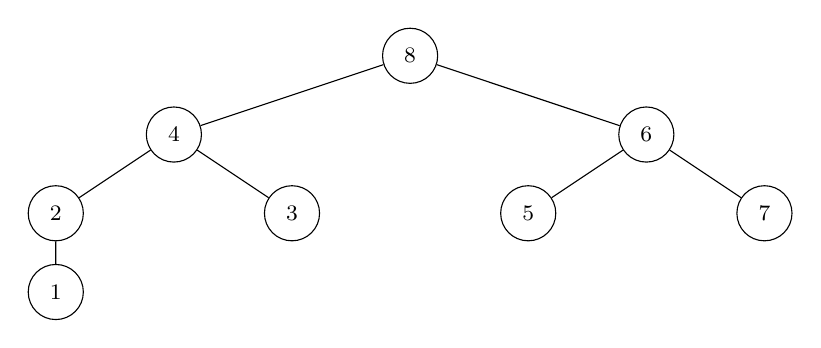
\begin{tikzpicture}[
      level distance=1cm,
      level 1/.style={sibling distance=6cm},
      level 2/.style={sibling distance=3cm},
      level 3/.style={sibling distance=1.5cm},
      every node/.style={circle, draw, minimum size=0.7cm, font=\footnotesize}
    ]
      \node {8}
        child {node {4}
          child {node {2}
            child {node {1}}
          }
          child {node {3}}
        }
        child {node {6}
          child {node {5}}
          child {node {7}}
        };
    \end{tikzpicture}
  \end{center}

  \vspace{0.3cm}
  \small
  \textbf{Navigation:}
  \begin{itemize}
    \item Parent: i + LSB(i) (move up)
    \item Previous range: i - LSB(i) (move left)
  \end{itemize}
\end{frame}

\section{Core Operations}

\begin{frame}[fragile]{Point Update}
  \textbf{Add delta to element at index i}

  \begin{lstlisting}[language=Python, basicstyle=\ttfamily\footnotesize]
def update(self, i, delta):
    """Add delta to element at index i (1-indexed)"""
    while i <= self.n:
        self.tree[i] += delta
        i += i & (-i)  # Move to parent
  \end{lstlisting}

  \vspace{0.5cm}
  \textbf{How it works:}
  \begin{enumerate}
    \item Start at index i
    \item Update current node
    \item Move to parent by adding LSB: i += LSB(i)
    \item Repeat until out of bounds
  \end{enumerate}

  \vspace{0.5cm}
  \textbf{Time Complexity:} O(log n)
  \begin{itemize}
    \item At most $\log_2(n)$ iterations
    \item Each iteration: O(1) operations
  \end{itemize}
\end{frame}

\begin{frame}{Update Example}
  \textbf{Update index 5 with delta = 3}

  \vspace{0.3cm}
  \textbf{Steps:}
  \begin{enumerate}
    \item i = 5, LSB(5) = 1
      \begin{itemize}
        \item \texttt{tree[5] += 3}
        \item Next: 5 + 1 = 6
      \end{itemize}
    \item i = 6, LSB(6) = 2
      \begin{itemize}
        \item \texttt{tree[6] += 3}
        \item Next: 6 + 2 = 8
      \end{itemize}
    \item i = 8, LSB(8) = 8
      \begin{itemize}
        \item \texttt{tree[8] += 3}
        \item Next: 8 + 8 = 16 (stop if n < 16)
      \end{itemize}
  \end{enumerate}

  \vspace{0.5cm}
  \textbf{Result:} Updated 3 nodes in O(log n) time!

  \vspace{0.3cm}
  These nodes represent all ranges containing index 5.
\end{frame}

\begin{frame}[fragile]{Prefix Sum Query}
  \textbf{Get sum from index 1 to i}

  \begin{lstlisting}[language=Python, basicstyle=\ttfamily\footnotesize]
def prefix_sum(self, i):
    """Get sum of elements from index 1 to i (1-indexed)"""
    result = 0
    while i > 0:
        result += self.tree[i]
        i -= i & (-i)  # Move to previous range
    return result
  \end{lstlisting}

  \vspace{0.5cm}
  \textbf{How it works:}
  \begin{enumerate}
    \item Start at index i
    \item Add current node's value to result
    \item Move to previous non-overlapping range: i -= LSB(i)
    \item Repeat until i = 0
  \end{enumerate}

  \vspace{0.5cm}
  \textbf{Time Complexity:} O(log n)
\end{frame}

\begin{frame}{Prefix Sum Example}
  \textbf{Query: prefix\_sum(13)}

  \vspace{0.3cm}
  \textbf{Steps:}
  \begin{enumerate}
    \item i = 13, LSB(13) = 1
      \begin{itemize}
        \item \texttt{result += tree[13]} (covers [13])
        \item Next: 13 - 1 = 12
      \end{itemize}
    \item i = 12, LSB(12) = 4
      \begin{itemize}
        \item \texttt{result += tree[12]} (covers [9-12])
        \item Next: 12 - 4 = 8
      \end{itemize}
    \item i = 8, LSB(8) = 8
      \begin{itemize}
        \item \texttt{result += tree[8]} (covers [1-8])
        \item Next: 8 - 8 = 0 (stop)
      \end{itemize}
  \end{enumerate}

  \vspace{0.5cm}
  \textbf{Ranges summed:} [13] + [9-12] + [1-8] = [1-13] \checkmark
\end{frame}

\begin{frame}[fragile]{Range Sum Query}
  \textbf{Get sum from index l to r}

  \begin{lstlisting}[language=Python, basicstyle=\ttfamily\footnotesize]
def range_sum(self, left, right):
    """Sum from left to right (1-indexed, inclusive)"""
    return self.prefix_sum(right) - self.prefix_sum(left - 1)
  \end{lstlisting}

  \vspace{0.5cm}
  \textbf{Key Insight:}
  \begin{itemize}
    \item sum[l..r] = sum[1..r] - sum[1..l-1]
    \item Uses inclusion-exclusion principle
    \item Works because sum is invertible (subtraction defined)
  \end{itemize}

  \vspace{0.5cm}
  \textbf{Example:}
  \begin{lstlisting}[language=Python, basicstyle=\ttfamily\footnotesize]
# Query sum from index 3 to 7
sum[3..7] = prefix_sum(7) - prefix_sum(2)
  \end{lstlisting}

  \vspace{0.3cm}
  \textbf{Time Complexity:} O(log n) - two prefix sum queries
\end{frame}

\begin{frame}[fragile]{Complete Implementation}
  \begin{lstlisting}[language=Python, basicstyle=\ttfamily\footnotesize]
class FenwickTree:
    def __init__(self, n):
        self.n = n
        self.tree = [0] * (n + 1)  # 1-indexed

    def update(self, i, delta):
        """Add delta to index i (1-indexed)"""
        while i <= self.n:
            self.tree[i] += delta
            i += i & (-i)

    def prefix_sum(self, i):
        """Sum from index 1 to i (1-indexed)"""
        result = 0
        while i > 0:
            result += self.tree[i]
            i -= i & (-i)
        return result

    def range_sum(self, left, right):
        """Sum from left to right (1-indexed)"""
        return self.prefix_sum(right) - self.prefix_sum(left - 1)
  \end{lstlisting}

  \textbf{That's it! ~20 lines for powerful data structure}
\end{frame}

\section{Building the Tree}

\begin{frame}[fragile]{Initialization from Array}
  \textbf{Two approaches to build tree from array:}

  \vspace{0.3cm}
  \textbf{Method 1: Using update (Simple but slower)}
  \begin{lstlisting}[language=Python, basicstyle=\ttfamily\footnotesize]
def __init__(self, arr):
    self.n = len(arr)
    self.tree = [0] * (self.n + 1)
    for i in range(self.n):
        self.update(i + 1, arr[i])
  \end{lstlisting}

  \textbf{Time:} O(n log n)

  \vspace{0.5cm}
  \textbf{Method 2: Direct construction (Optimized)}
  \begin{lstlisting}[language=Python, basicstyle=\ttfamily\footnotesize]
def build_fast(arr):
    n = len(arr)
    tree = [0] * (n + 1)
    for i in range(1, n + 1):
        tree[i] += arr[i - 1]
        j = i + (i & -i)  # Parent index
        if j <= n:
            tree[j] += tree[i]
    return tree
  \end{lstlisting}

  \textbf{Time:} O(n) - much faster!
\end{frame}

\begin{frame}{Build Process Visualization}
  \textbf{Direct O(n) construction:}

  \vspace{0.3cm}
  For each index i:
  \begin{enumerate}
    \item Copy array value to tree[i]
    \item Find parent: j = i + LSB(i)
    \item Add tree[i] to tree[j]
  \end{enumerate}

  \vspace{0.5cm}
  \textbf{Why this works:}
  \begin{itemize}
    \item Process indices in increasing order
    \item When processing index i, all children already processed
    \item Parent inherits sum from child
    \item Each index processed exactly once: O(n)
  \end{itemize}

  \vspace{0.5cm}
  \textbf{Comparison:}
  \begin{itemize}
    \item O(n log n): Easy to understand, uses existing update()
    \item O(n): More efficient, clever bottom-up approach
  \end{itemize}
\end{frame}

\section{Advanced Techniques}

\begin{frame}[fragile]{Range Updates}
  \textbf{Problem:} Add delta to all elements in range [l, r]

  \vspace{0.3cm}
  \textbf{Solution:} Use difference array technique

  \begin{lstlisting}[language=Python, basicstyle=\ttfamily\footnotesize]
class FenwickTreeRangeUpdate:
    def __init__(self, n):
        self.n = n
        self.tree = [0] * (n + 1)

    def range_update(self, left, right, delta):
        """Add delta to all elements in [left, right]"""
        self.update(left, delta)
        self.update(right + 1, -delta)

    def point_query(self, i):
        """Get value at index i after all updates"""
        return self.prefix_sum(i)
  \end{lstlisting}

  \vspace{0.5cm}
  \textbf{Key Idea:}
  \begin{itemize}
    \item Store differences instead of values
    \item Range update becomes two point updates
    \item Point query uses prefix sum
  \end{itemize}
\end{frame}

\begin{frame}{Range Update Example}
  \textbf{Add 5 to range [3, 6]}

  \vspace{0.3cm}
  Initial array: [0, 0, 0, 0, 0, 0, 0, 0]

  \vspace{0.5cm}
  \textbf{Operations:}
  \begin{enumerate}
    \item \texttt{update(3, 5)} - Mark start of range
    \item \texttt{update(7, -5)} - Mark end of range
  \end{enumerate}

  \vspace{0.5cm}
  \textbf{Difference array:} [0, 0, 5, 0, 0, 0, -5, 0]

  \vspace{0.3cm}
  \textbf{Prefix sums (actual values):}
  \begin{itemize}
    \item Index 1: 0
    \item Index 2: 0
    \item Index 3: 0 + 5 = 5
    \item Index 4: 5
    \item Index 5: 5
    \item Index 6: 5
    \item Index 7: 5 + (-5) = 0
    \item Index 8: 0
  \end{itemize}

  \textbf{Result:} [0, 0, 5, 5, 5, 5, 0, 0] \checkmark
\end{frame}

\begin{frame}[fragile]{2D Fenwick Tree}
  \textbf{For 2D range sum queries}

  \begin{lstlisting}[language=Python, basicstyle=\ttfamily\tiny]
class FenwickTree2D:
    def __init__(self, rows, cols):
        self.rows = rows
        self.cols = cols
        self.tree = [[0] * (cols + 1) for _ in range(rows + 1)]

    def update(self, row, col, delta):
        """Add delta to cell (row, col)"""
        i = row
        while i <= self.rows:
            j = col
            while j <= self.cols:
                self.tree[i][j] += delta
                j += j & (-j)
            i += i & (-i)

    def prefix_sum(self, row, col):
        """Sum of rectangle from (1,1) to (row, col)"""
        result = 0
        i = row
        while i > 0:
            j = col
            while j > 0:
                result += self.tree[i][j]
                j -= j & (-j)
            i -= i & (-i)
        return result

    def range_sum(self, r1, c1, r2, c2):
        """Sum of rectangle from (r1,c1) to (r2,c2)"""
        return (self.prefix_sum(r2, c2) - self.prefix_sum(r1-1, c2)
                - self.prefix_sum(r2, c1-1) + self.prefix_sum(r1-1, c1-1))
  \end{lstlisting}
\end{frame}

\begin{frame}{2D Range Sum}
  \textbf{Query rectangle sum using inclusion-exclusion}

  \vspace{0.3cm}
  \textbf{Sum of rectangle (r1, c1) to (r2, c2):}

  \begin{center}
    \texttt{sum = A - B - C + D}
  \end{center}

  \vspace{0.3cm}
  Where:
  \begin{itemize}
    \item A = prefix\_sum(r2, c2) - full rectangle to (r2, c2)
    \item B = prefix\_sum(r1-1, c2) - top portion (subtract)
    \item C = prefix\_sum(r2, c1-1) - left portion (subtract)
    \item D = prefix\_sum(r1-1, c1-1) - overlap (add back)
  \end{itemize}

  \vspace{0.5cm}
  \textbf{Complexity:}
  \begin{itemize}
    \item Update: O(log m $\times$ log n)
    \item Query: O(log m $\times$ log n)
    \item Space: O(m $\times$ n)
  \end{itemize}
\end{frame}

\section{Comparison with Segment Trees}

\begin{frame}{Fenwick vs Segment Tree}
  \begin{table}
    \centering
    \small
    \begin{tabular}{|l|c|c|}
      \hline
      \textbf{Feature} & \textbf{Fenwick Tree} & \textbf{Segment Tree} \\
      \hline
      Space & O(n) & O(4n) \\
      \hline
      Update & O(log n) & O(log n) \\
      \hline
      Query & O(log n) & O(log n) \\
      \hline
      Construction & O(n) or O(n log n) & O(n) \\
      \hline
      Code Lines & ~20 & ~50 \\
      \hline
      Operations & Sum, XOR & Any associative \\
      \hline
      Range Update & Difference array & Lazy propagation \\
      \hline
      Simplicity & Simple & Moderate \\
      \hline
      Constants & Lower & Higher \\
      \hline
    \end{tabular}
  \end{table}

  \vspace{0.5cm}
  \textbf{Key Difference:} Fenwick Tree requires invertible operations!
\end{frame}

\begin{frame}{When to Use Each}
  \textbf{Use Fenwick Tree when:}
  \begin{itemize}
    \item Operation is invertible (sum, XOR)
    \item Want minimal memory usage
    \item Prefer simple implementation
    \item Competitive programming (faster to code)
    \item Range sum queries with updates
  \end{itemize}

  \vspace{0.5cm}
  \textbf{Use Segment Tree when:}
  \begin{itemize}
    \item Need range min/max queries
    \item Operation not invertible (min, max, GCD)
    \item Need lazy propagation
    \item Need to store extra data per node
    \item More complex range operations
  \end{itemize}

  \vspace{0.5cm}
  \textbf{Example where Fenwick fails:}
  \begin{itemize}
    \item Range minimum: min(a,b) - min(c,d) is meaningless!
    \item Must use Segment Tree or Sparse Table
  \end{itemize}
\end{frame}

\begin{frame}{Performance Comparison}
  \textbf{Benchmark: 1,000,000 elements}

  \vspace{0.3cm}
  \begin{table}
    \centering
    \begin{tabular}{|l|r|r|}
      \hline
      \textbf{Metric} & \textbf{Fenwick Tree} & \textbf{Segment Tree} \\
      \hline
      Memory & 4 MB & 16 MB \\
      \hline
      Build time & ~20 ms & ~15 ms \\
      \hline
      1M updates & ~50 ms & ~80 ms \\
      \hline
      1M queries & ~50 ms & ~80 ms \\
      \hline
      Code size & ~20 lines & ~50 lines \\
      \hline
    \end{tabular}
  \end{table}

  \vspace{0.5cm}
  \textbf{Advantages of Fenwick:}
  \begin{itemize}
    \item 4x less memory
    \item 1.6x faster for updates/queries
    \item 2.5x less code
    \item Better cache performance
  \end{itemize}
\end{frame}

\section{Common Patterns \& Pitfalls}

\begin{frame}[fragile]{Pattern: Counting Inversions}
  \textbf{Problem:} Count pairs (i, j) where i < j but arr[i] > arr[j]

  \begin{lstlisting}[language=Python, basicstyle=\ttfamily\tiny]
def count_inversions(arr):
    # Coordinate compression
    sorted_arr = sorted(set(arr))
    rank = {v: i+1 for i, v in enumerate(sorted_arr)}

    bit = FenwickTree(len(sorted_arr))
    inversions = 0

    # Process from right to left
    for i in range(len(arr) - 1, -1, -1):
        r = rank[arr[i]]
        # Count elements smaller than arr[i] seen so far
        inversions += bit.prefix_sum(r - 1)
        # Mark current element as seen
        bit.update(r, 1)

    return inversions
  \end{lstlisting}

  \vspace{0.3cm}
  \textbf{Time Complexity:} O(n log n)

  \vspace{0.3cm}
  \textbf{Applications:}
  \begin{itemize}
    \item Sorting analysis
    \item Ranking systems
    \item Measuring disorder in sequences
  \end{itemize}
\end{frame}

\begin{frame}{Common Pitfalls}
  \textbf{1. Index Confusion (0 vs 1-indexed)}
  \begin{itemize}
    \item Fenwick Tree is 1-indexed!
    \item Index 0 unused or sentinel
    \item Always convert: \texttt{update(i + 1, delta)}
  \end{itemize}

  \vspace{0.3cm}
  \textbf{2. Using for Non-Invertible Operations}
  \begin{itemize}
    \item Cannot do range min/max with Fenwick
    \item Subtraction doesn't work: min(a,b) - min(c,d)
    \item Use Segment Tree instead
  \end{itemize}

  \vspace{0.3cm}
  \textbf{3. Incorrect Size}
  \begin{itemize}
    \item Array size must be n+1 (index 0 to n)
    \item Check bounds in update loop
  \end{itemize}

  \vspace{0.3cm}
  \textbf{4. Forgetting Negative Values}
  \begin{itemize}
    \item Fenwick requires positive indices
    \item Use coordinate compression for negative values
  \end{itemize}
\end{frame}

\begin{frame}[fragile]{Pitfall Examples}
  \textbf{Wrong: 0-indexed usage}
  \begin{lstlisting}[language=Python, basicstyle=\ttfamily\footnotesize]
bit = FenwickTree(n)
bit.update(0, 5)  # ERROR! Index 0 is invalid
  \end{lstlisting}

  \textbf{Correct: Convert to 1-indexed}
  \begin{lstlisting}[language=Python, basicstyle=\ttfamily\footnotesize]
bit = FenwickTree(n)
bit.update(1, 5)  # OK: Update first element
  \end{lstlisting}

  \vspace{0.5cm}
  \textbf{Wrong: Range minimum}
  \begin{lstlisting}[language=Python, basicstyle=\ttfamily\footnotesize]
# Cannot use Fenwick for this!
min_val = bit.range_sum(l, r)  # Meaningless for min
  \end{lstlisting}

  \textbf{Correct: Use Segment Tree}
  \begin{lstlisting}[language=Python, basicstyle=\ttfamily\footnotesize]
seg_tree = SegmentTree(arr)
min_val = seg_tree.range_min(l, r)  # OK
  \end{lstlisting}
\end{frame}

\begin{frame}{Debugging Tips}
  \textbf{How to debug Fenwick Tree issues:}

  \vspace{0.3cm}
  \begin{enumerate}
    \item \textbf{Print tree array}
      \begin{itemize}
        \item Visualize internal state
        \item Check if values make sense
      \end{itemize}

    \item \textbf{Verify LSB calculation}
      \begin{itemize}
        \item Test: \texttt{i \& (-i)}
        \item Check against manual calculation
      \end{itemize}

    \item \textbf{Check index conversions}
      \begin{itemize}
        \item 0-indexed input $\rightarrow$ 1-indexed tree
        \item Off-by-one errors common
      \end{itemize}

    \item \textbf{Test with small arrays}
      \begin{itemize}
        \item Use n = 4 or 8 for manual verification
        \item Compare with brute force
      \end{itemize}

    \item \textbf{Validate bounds}
      \begin{itemize}
        \item Ensure i $\leq$ n in update
        \item Ensure i > 0 in prefix\_sum
      \end{itemize}
  \end{enumerate}
\end{frame}

\section{Applications}

\begin{frame}[fragile]{Application 1: Range Sum Query}
  \textbf{LeetCode 307: Range Sum Query - Mutable}

  \begin{lstlisting}[language=Python, basicstyle=\ttfamily\footnotesize]
class NumArray:
    def __init__(self, nums):
        self.nums = nums
        self.n = len(nums)
        self.tree = [0] * (self.n + 1)
        for i in range(self.n):
            self._update(i + 1, nums[i])

    def update(self, index, val):
        delta = val - self.nums[index]
        self.nums[index] = val
        self._update(index + 1, delta)

    def _update(self, i, delta):
        while i <= self.n:
            self.tree[i] += delta
            i += i & (-i)

    def sumRange(self, left, right):
        return self._prefix_sum(right + 1) - self._prefix_sum(left)

    def _prefix_sum(self, i):
        result = 0
        while i > 0:
            result += self.tree[i]
            i -= i & (-i)
        return result
  \end{lstlisting}
\end{frame}

\begin{frame}[fragile]{Application 2: Count Smaller Numbers}
  \textbf{LeetCode 315: Count of Smaller Numbers After Self}

  \begin{lstlisting}[language=Python, basicstyle=\ttfamily\tiny]
def countSmaller(nums):
    # Coordinate compression
    sorted_nums = sorted(set(nums))
    rank = {v: i+1 for i, v in enumerate(sorted_nums)}

    bit = FenwickTree(len(sorted_nums))
    result = []

    # Process from right to left
    for num in reversed(nums):
        r = rank[num]
        # Count numbers smaller than current
        count = bit.prefix_sum(r - 1)
        result.append(count)
        # Mark current number as seen
        bit.update(r, 1)

    return result[::-1]

class FenwickTree:
    def __init__(self, n):
        self.n = n
        self.tree = [0] * (n + 1)

    def update(self, i, delta):
        while i <= self.n:
            self.tree[i] += delta
            i += i & (-i)

    def prefix_sum(self, i):
        result = 0
        while i > 0:
            result += self.tree[i]
            i -= i & (-i)
        return result
  \end{lstlisting}
\end{frame}

\begin{frame}[fragile]{Application 3: 2D Matrix Range Sum}
  \textbf{LeetCode 308: Range Sum Query 2D - Mutable}

  \begin{lstlisting}[language=Python, basicstyle=\ttfamily\tiny]
class NumMatrix:
    def __init__(self, matrix):
        if not matrix or not matrix[0]:
            return
        self.matrix = matrix
        self.rows = len(matrix)
        self.cols = len(matrix[0])
        self.tree = [[0] * (self.cols + 1) for _ in range(self.rows + 1)]

        for i in range(self.rows):
            for j in range(self.cols):
                self._update(i + 1, j + 1, matrix[i][j])

    def update(self, row, col, val):
        delta = val - self.matrix[row][col]
        self.matrix[row][col] = val
        self._update(row + 1, col + 1, delta)

    def _update(self, row, col, delta):
        i = row
        while i <= self.rows:
            j = col
            while j <= self.cols:
                self.tree[i][j] += delta
                j += j & (-j)
            i += i & (-i)

    def sumRegion(self, r1, c1, r2, c2):
        return (self._prefix_sum(r2+1, c2+1) - self._prefix_sum(r1, c2+1)
                - self._prefix_sum(r2+1, c1) + self._prefix_sum(r1, c1))

    def _prefix_sum(self, row, col):
        result, i = 0, row
        while i > 0:
            j = col
            while j > 0:
                result += self.tree[i][j]
                j -= j & (-j)
            i -= i & (-i)
        return result
  \end{lstlisting}
\end{frame}

\begin{frame}{Real-World Usage}
  \textbf{Competitive Programming:}
  \begin{itemize}
    \item Codeforces: Preferred for speed
    \item AtCoder: Common in range query problems
    \item ICPC: Quick to implement under time pressure
  \end{itemize}

  \vspace{0.5cm}
  \textbf{Production Systems:}
  \begin{itemize}
    \item Analytics databases (OLAP)
    \item Time-series aggregation
    \item Real-time monitoring dashboards
    \item Financial tick data analysis
  \end{itemize}

  \vspace{0.5cm}
  \textbf{Advanced Applications:}
  \begin{itemize}
    \item Persistent Fenwick Trees (versioned queries)
    \item Parallel updates (lock-free concurrent operations)
    \item Compressed Fenwick Trees (sparse arrays)
    \item Multi-dimensional (3D, 4D spatial queries)
  \end{itemize}
\end{frame}

\section{Summary}

\begin{frame}{Summary: Key Concepts}
  \textbf{Fenwick Tree Fundamentals:}
  \begin{itemize}
    \item Array-based structure using binary representation
    \item LSB determines responsibility ranges
    \item Navigation via bit manipulation: i $\pm$ LSB(i)
  \end{itemize}

  \vspace{0.5cm}
  \textbf{Core Operations:}
  \begin{itemize}
    \item Update: O(log n) - add delta, move to parents
    \item Prefix sum: O(log n) - accumulate, move to previous ranges
    \item Range sum: O(log n) - difference of prefix sums
  \end{itemize}

  \vspace{0.5cm}
  \textbf{Key Properties:}
  \begin{itemize}
    \item Space: O(n) - minimal overhead
    \item Simple: ~20 lines of code
    \item Fast: Lower constants than Segment Tree
    \item Limitation: Requires invertible operations
  \end{itemize}
\end{frame}

\begin{frame}{Summary: Comparison}
  \begin{table}
    \centering
    \footnotesize
    \begin{tabular}{|l|c|c|c|}
      \hline
      \textbf{Structure} & \textbf{Space} & \textbf{Ops} & \textbf{Operations Supported} \\
      \hline
      Array & O(n) & O(n)/O(1) & All \\
      Prefix Sum & O(n) & O(n)/O(1) & Invertible \\
      Sqrt Decomp & O(n) & O($\sqrt{n}$) & All \\
      \textbf{Fenwick} & \textbf{O(n)} & \textbf{O(log n)} & \textbf{Invertible} \\
      Segment Tree & O(4n) & O(log n) & All associative \\
      Sparse Table & O(n log n) & O(log n)/O(1) & Idempotent \\
      \hline
    \end{tabular}
  \end{table}

  \vspace{0.5cm}
  \textbf{Sweet Spot:}
  \begin{itemize}
    \item Best for range sum queries
    \item Optimal space-time trade-off
    \item Simplest code among log(n) structures
  \end{itemize}
\end{frame}

\begin{frame}{Key Takeaways}
  \begin{enumerate}
    \item Fenwick Trees are elegant and efficient
    \item Bit manipulation enables O(log n) operations
    \item 1-indexed convention simplifies LSB logic
    \item Perfect for invertible operations (sum, XOR)
    \item Cannot handle min/max - use Segment Tree
    \item Simpler and faster than Segment Tree when applicable
    \item Essential tool for competitive programming
    \item Useful in production for analytics systems
  \end{enumerate}

  \vspace{0.5cm}
  \textbf{Remember:}
  \begin{itemize}
    \item Always check if operation is invertible
    \item Master bit manipulation: \texttt{i \& (-i)}
    \item Watch out for 0-indexed vs 1-indexed
    \item O(n) construction is possible and recommended
  \end{itemize}
\end{frame}

\begin{frame}{Practice Problems}
  \textbf{LeetCode:}
  \begin{itemize}
    \item 307. Range Sum Query - Mutable
    \item 308. Range Sum Query 2D - Mutable
    \item 315. Count of Smaller Numbers After Self
    \item 327. Count of Range Sum
    \item 493. Reverse Pairs
  \end{itemize}

  \vspace{0.5cm}
  \textbf{Codeforces:}
  \begin{itemize}
    \item Fenwick tree problems (rated 1400-2000)
    \item Range query contests
    \item Dynamic programming with BIT
  \end{itemize}

  \vspace{0.5cm}
  \textbf{Skills to Practice:}
  \begin{itemize}
    \item Coordinate compression
    \item 2D Fenwick Trees
    \item Range updates with difference arrays
    \item Combining with other algorithms
  \end{itemize}
\end{frame}

\begin{frame}{Further Learning}
  \textbf{Advanced Topics:}
  \begin{itemize}
    \item Persistent Fenwick Trees
    \item Parallel/Concurrent Fenwick Trees
    \item Range updates with range queries
    \item Fenwick Tree on trees (Heavy-Light Decomposition)
    \item Offline query optimization
  \end{itemize}

  \vspace{0.5cm}
  \textbf{Resources:}
  \begin{itemize}
    \item CP-Algorithms: Binary Indexed Tree tutorial
    \item Topcoder: Range query structures
    \item Codeforces: Educational rounds on BIT
    \item "Competitive Programmer's Handbook"
  \end{itemize}

  \vspace{0.5cm}
  \textbf{Related Structures:}
  \begin{itemize}
    \item Segment Trees
    \item Sqrt Decomposition
    \item Sparse Table
    \item Wavelet Trees
  \end{itemize}
\end{frame}

\begin{frame}
  \begin{center}
    {\Huge Thank You!}

    \vspace{1cm}
    {\Large Questions?}

    \vspace{1cm}
    \textit{Fenwick Trees: Simplicity meets Efficiency}
  \end{center}
\end{frame}

\end{document}
